\documentclass{beamer}

\mode<presentation> {

%\usetheme{default}
\usetheme{Rochester}
\usecolortheme{lily}

\setbeamertemplate{footline}[page number] 
\beamertemplatenavigationsymbolsempty
\setbeamertemplate{bibliography item}{} %Remove icons in bibliography
}

\usepackage{graphicx} % Allows including images
\usepackage{amsmath}
\usepackage{lmodern}
\usepackage{listings}

\lstset{
    language=[5.0]Lua,
    basicstyle=\fontsize{11}{9},
    sensitive=true,
    breaklines=true,
    tabsize=2
}

%----------------------------------------------------------------------------------------
%	TITLE PAGE
%----------------------------------------------------------------------------------------

\title[Project Learning Systems]{Unsupervised training of Convolutional Networks with SGVB} 

\author{Joost van Amersfoort \& Otto Fabius} 
\institute[UvA] 
{University of Amsterdam
Supervisor: Diederik Kingma
\medskip
}
\date{\today} % Date, can be changed to a custom date

\begin{document}

\begin{frame}
\titlepage % Print the title page as the first slide
\end{frame}

\begin{frame}
\frametitle{Overview}
\tableofcontents 
\end{frame}

%----------------------------------------------------------------------------------------
%	PRESENTATION SLIDES
%----------------------------------------------------------------------------------------

\section{Introduction}


\begin{frame}
\frametitle{Introduction}
\begin{itemize}
	\item Convolutional Networks have had much success recently in Computer Vision tasks, due to an increase in computing power and available annotated data and efficient GPU implementations
	\item Currently there are no successful means of training such networks unsupervised has been reported
	\item The recently developed SGVB makes efficient, effective Bayesian Inference possible by means of stochastic gradient descent. This can be used to train a Convolution Neural Network unsupervised
\end{itemize}
\end{frame}

\section{Theory}

\subsection{Convolutional Neural Networks}
\begin{frame}
\frametitle{Convolutional Neural Networks - Error Backpropagation}
The gradient of a convolution is relatively straightforward.\\ Let $L$ be the loss function, and $y = x * k$ the convolution operation with weights $W$, then \\   

\begin{align*}
\nabla_W L = (\nabla_y L) * x^T 
\end{align*}

\end{frame}

\begin{frame}
\frametitle{Convolutional Neural Networks - Example structure}

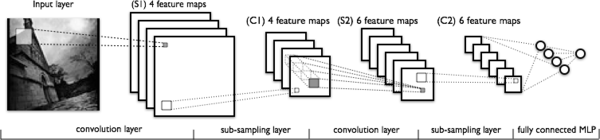
\includegraphics[scale = 0.7]{img/convnet.png} \\\cite{farabet2014}

%image of example structure
%tell something about need for computational resources
\end{frame}

\subsection{SGVB}
\begin{frame}
\frametitle{Unsupervised Training with SGVB}
%image of example structure with latent variables and deconvolution
Model $P(\mathbf{X},\mathbf{Z}) = \frac{P(\mathbf{Z})\cdot P(\mathbf{X}|\mathbf{Z})}{P(\mathbf{Z}|\mathbf{X})}$ to find structure in data $\mathbf{X}$. \vspace{0.5mm}
Here, $P(\mathbf{X}|\mathbf{Z})$ is the deconvolutional layer and the intractable $P(\mathbf{Z}|\mathbf{X})$ is approximated by $q(\mathbf{Z}|\mathbf{X})$, which is the Convolutional layer.
%mention that we need to train the parameters of the network and that we can use this for pretraining an convnet, but also have a generative model which can be used for many different tasks.
\end{frame}

\begin{frame}
\frametitle{Marginal Likelihood as Optimization Criterion}
%Of course, we want to learn the parameters via gradient descent on some objective function. %Mention work by Kingma and Welling, add reference
The marginal probability of $\mathbf{X}$ can be written as:
\begin{align*}
\log p_\theta(\mathbf{X}) = D_{KL}(q_\phi(\mathbf{Z}|\mathbf{X}) || p_\theta(\mathbf{Z}|\mathbf{X})) + \mathcal{L}(\mathbf{\theta}, \mathbf{\phi}; \mathbf{X})
\end{align*}
Where 
$\mathcal{L}(\mathbf{\theta}, \mathbf{\phi}; \mathbf{X})$
is the \textit{lower bound} on the marginal likelihood
$
P(\mathbf{X}) = \int_z P(\mathbf{Z})P(\mathbf{X}|\mathbf{Z})d\mathbf{Z}$
\end{frame}

\begin{frame}
\frametitle{Reparameterization}
We need to estimate (stochastic) gradients w.r.t the model parameters. For this, we reparameterize $q(\mathbf{Z}|\mathbf{X})$ as a differentiable, deterministic function $g_{\theta}(\epsilon,\mathbf{x})$, which depends on sampled noise $\epsilon \sim N(0,1)$. \\ Now if we sample $\tilde{z} \sim q(\mathbf{Z}|\mathbf{X})$, $logp_{\theta}(\mathbf{X})$ is fully differentiable and we can perform stochastic gradient descent on the model parameters!
\end{frame}

\section{Research Questions}
\begin{frame}
\frametitle{Research Questions}
\begin{enumerate}
	\item How can we perform Deconvolution?
	\item What architectures are effective and efficient?
	\item How well do trained Convolutional Networks model the data, compared to fully connected models?
\end{enumerate}
\end{frame}

\section{Implementation}

\subsection{Torch7}
\begin{frame}
\frametitle{Implementation using \href{http://torch.ch/}{Torch7}}
\begin{itemize}
	\item Torch7 is a framework on top of Lua, utilizing the LuaJIT and crucial parts are in C/CUDA code
	\item Models in Torch7 consist of a stack of modules (layers), e.g. Sigmoid, Linear and Convolution
	\item A module consists roughly of three functions:
		\begin{itemize}
			\item updateInput, which defines how the input is updated
			\item updateGradOutput, which defines how the gradient is updated during Backpropagation
			\item AccGradParameters, which defines how the parameters of the module are updated, given the gradient
		\end{itemize}
\end{itemize}
\end{frame}

\begin{frame}[fragile]
\frametitle{Example of model in Torch7}
\begin{lstlisting}
require 'torch'
require 'nn'

model = nn.Sequential()

-- stage 1 : standard convolution layer
model:add(nn.SpatialConvolution(1, 16, 5, 5))
model:add(nn.SpatialMaxPooling(2, 2, 2, 2))
model:add(nn.Sigmoid())

-- stage 2 : standard 2-layer neural network
model:add(nn.Linear(256, 128))
model:add(nn.Sigmoid())
model:add(nn.Linear(128,#classes))
\end{lstlisting}
\end{frame}


\begin{frame}
\frametitle{Example of model in Torch7}

\begin{itemize}
	\item Output of model can be used as input for a criterion, a seperate module
	\item Criterion outputs the error (used for keeping track of lowerbound) and a gradient of the error w.r.t to the input
	\item What rests is a simple \texttt{model:forward(batch)} and \texttt{model:backward(batch, error)}
\end{itemize}

\end{frame}

\begin{frame}
\frametitle{Using the GPU with Torch7}

\begin{itemize}
	\item All built-in modules support CUDA
	\item Custom modules (e.g. for reparametrization) required rewriting
	\item CUDA uses single precision instead of double, leads to numeric instability
	\item NVidia card necessary for CUDA (available on Amazon EC2 cloud)
\end{itemize}

\end{frame}

 
\section{Results}

%\begin{frame}
%\frametitle{How can we perform Deconvolution? - Option 1}
%% here figure of network, onlt the deconvolution part
%%describe upsampling and weight sharing
%Perform full deconvolution: 
%\begin{enumerate}
%\item Learn an NxN weight matrix (equal to the filtersize of the %convolutions) for each feature map to create an NxN window from %each pixel. 
%\item Reorganise the overlapping NxN windows to reconstruct a %feature map of the original dimensions.
%\end{enumerate}
%Restrictions:
%\begin{itemize}
%\item None, but this can not be done with the available modules in Torch7.
%\end{itemize} 
%explain that this is very restrictive
%\end{frame}

\begin{frame}
\frametitle{How can we perform Deconvolution? - Option 1}
% here figure of network, only the deconvolution part
Both the encoding layer and decoding layer consist of a convolution with $K$ $NxN$ filters with stride 1, after zero padding to keep the dimensions of the feature maps the same. \\ \vspace{4mm}
This approach prevents strides other than 1 and spatial max pooling. Although deeper networks often contain such layers, spatial max pooling or strides are desirable in ConvNets for multiple reasons and thus we need another method for deconvolution.

% explain why this is restrictive
\end{frame}

\begin{frame}
\frametitle{How can we perform Deconvolution? - Option 2}
%an image here would be simply awesome, otherwise we should probably draw this on the whiteboard.

Use a two-layer MLP with weight sharing to reconstruct the output. Each feature map ha its own set of weights, one for each unit in the hidden layer. Similarly, the hidden layer connects to the output with the same weight from each hidden unit to all pixels in a given feature map.
\\ \vspace{4mm}
This enables differences in spatial resolution in subsequent feature maps, but the factor between the two resolutions must be an integer.

%This is somewhat restrictive, but rarely a problem

%explain that the options have pros and cons, perhaps another slide on what worked best for a given architecture?
\end{frame}

\begin{frame}
\frametitle{Possible one layer architectures}

\begin{itemize}
	\item For one layer networks there are two options: with and without dimensionality reduction
	\item In an architecture without dimensionality reduction we perform zero padding with filter size - 1 before convolution. 
		\begin{itemize}
			\item Both encoder and decoder consist of padding and convolution layer
		\end{itemize}
	\item In an architecture with dimensionality reduction we use a convolution with a stride higher than 1 or a max 
	pooling layer
\end{itemize}

\end{frame}

\begin{frame}
\frametitle{Results of one layer architectures}
	\begin{itemize}
		\item Without dimensionality reduction gives UNKNOWN - ALIEN - THERE ARE NO ANSWERS HERE
		\item Dimensionality reduction using stride 2 leads to a lowerbound of -105 after convergence. This is similar to the result of the fully connected network of \cite{kingma2013stochastic}, with one third of the number of parameters and much faster convergence
		\item Dimensionality reduction using max pooling converges to a slightly higher lowerbound of -106. Showing that it's  harder to invert this operation.
	\end{itemize}
\end{frame}

\section{Discussion}


% %-----------------------------------------------
\begin{frame}{Bibliography}
	\nocite{*}
	\bibliographystyle{ieeetr}
	\bibliography{ref}
\end{frame}

%------------------------------------------------

\begin{frame}
\Huge{\centerline{Thank you for your attention!}}
\end{frame}

%----------------------------------------------------------------------------------------

\end{document} 
